
In our experiments, we evaluated our indexing techniques on two real world datasets. We have compared our indexing techniques by comparing the running time with that of the state of the art technique  . We are also concerned about the indexing time, especially for the M-tree index structure since we do not want our index procedure to run into hours.

The first dataset is the PubChem(-n and -b) dataset . The second dataset is from DUD, a directory of useful decoys for benchmarking virtual screening. DUD is provided by the Shoichet Laboratory in the Department of Pharmaceutical Chemistry at the University of California, San Francisco (UCSF). DUD is derived from ZINC, a database of commercially available compounds. To extract fingerprints we used MOLPRINT2D, a molecular fingerprinting technique.


\section{M-tree based Indexing analysis}	

For these set of experiments the test bed used was a 4 Intel(R) Core(TM) i7-4770 CPU \@ 3.40GHz with 8GB RAM. We have varied several parameters in the experiment and have tried to estimate them empirically. We have used the PubChem-n dataset for all analysis of the M-tree. We use different dataset sizes of 1000, 10,000 and 100,000 number of chemical compounds.

For evaluation purposes we implemented a linear brute force scan to compute the range query and used that as a benchmark for the results. The result set obtained from our technique was compared with the linear brute scan answer set for verification purposes using the fingerprint id's. The query time and the indexing time is averaged over the 500 random query sample data points and the unit in ms per compound. We have varied the following parameters .


\subsection{Limiting Outlier Set Size }

\begin{figure}[ht]	
\centering
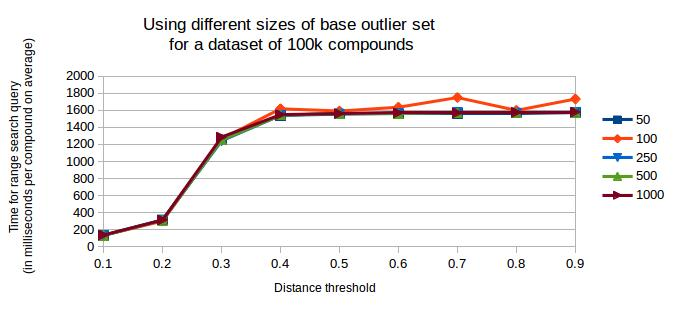
\includegraphics[width=1 \columnwidth]{img/image1.jpg}
\caption{M-tree: Average Range Query time versus Distance Threshold for various sizes of base outlier set}
\label{fig:5.1}
\end{figure}

Just to recap, it is the Minimum limiting size of the outlier set allowed (o). When the outlier set size falls below this limit, we terminate the indexing process.

As seen in \ref{fig:5.1} we can observe that the range search query time is almost constant with change in number of limiting outlier set size. We observed that the outlier base size did not have a significant effect on the query time for range search or on the number of comparisons. The indexing time increases with a lesser outlier base size because the depth of the M-tree increases . The algorithm is applied recursively on the outlier sets, hence when we have a lower base size limit for the outlier sets the number of times the recursion is applied is greater. Since we did not see a great change in query time or number of comparisons we have fixed the size the outlier size limit to 1/100th of the dataset size for all the future experiments.


\begin{figure}[ht!]	
\centering
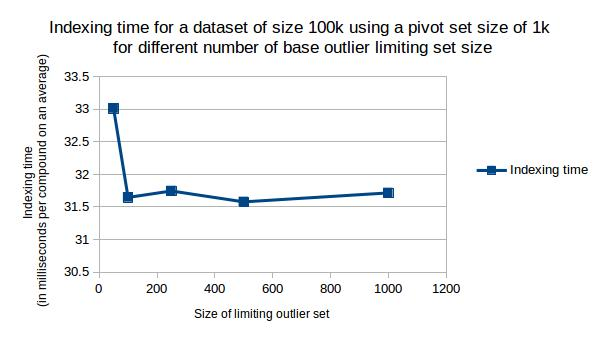
\includegraphics[width=1 \columnwidth]{img/image8.jpg}
\caption{M-tree: Indexing time versus different sizes of base limiting outlier set}
\label{fig:5.2}
\end{figure}


Ideally, indexing time should decrease with increase in number of limiting outlier size. This is because the depth of the M-tree grows with increase in the limiting size of the outlier set. The indexing process is a recursive procedure and termination occurs only when the size of the outlier set falls below the given limiting size. Hence in normal circumstances the indexing time must decrease as we increase the limiting size, but as seen in \autoref{fig:5.2} the decrease is minimal and changing \textit{o} doesn't change the indexing time much. 






\subsection{Pivot Set size}
The pivot set size as described earlier is the number of random pivots chosen at each step of the indexing process (p). \textit{p} determines the number of nodes at every level of the index structure. The number of nodes at each level is equal to p+1.

\autoref{fig:5.3},\autoref{fig:5.4},\autoref{fig:5.5}  show how the range search query time varies versus different distance threshold for different sizes of the pivot set for databases of size 1,000 , 10,000 and 100,000 compounds respectively. We can observe the time is almost similar at high threshold values for different number of pivots. For low threshold values we are successfully able to prune away all many nodes using triangle inequality. 


\begin{figure}[ht!]	
\centering
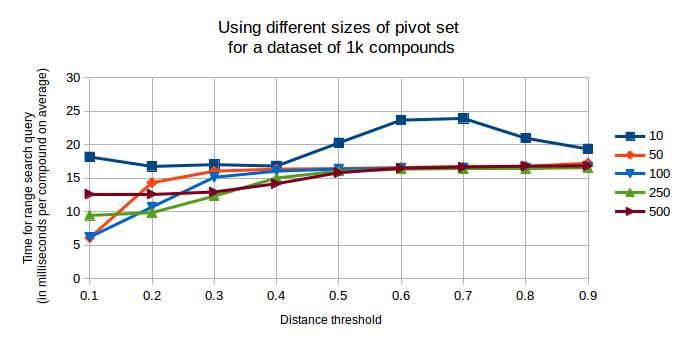
\includegraphics[width=1 \columnwidth]{img/image2.jpg}
\caption{M-tree: Average Range Query time versus Distance Threshold for various sizes of pivot set - 1k PubChem-n database}
\label{fig:5.3}
\end{figure}


\begin{figure}[ht!]	
\centering
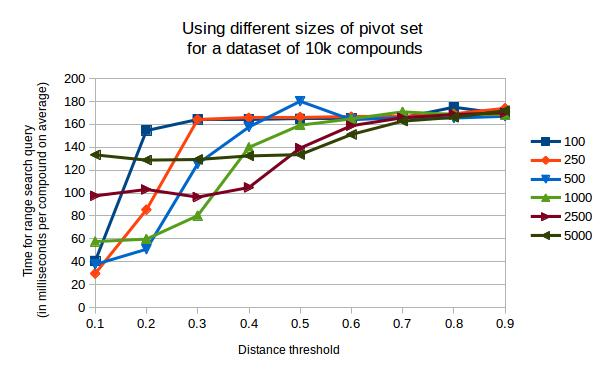
\includegraphics[width=1 \columnwidth]{img/image3.jpg}
\caption{M-tree: Average Range Query time versus Distance Threshold for various sizes of pivot set - 10k PubChem-n database}
\label{fig:5.4}
\end{figure}


\begin{figure}[ht!]	
\centering
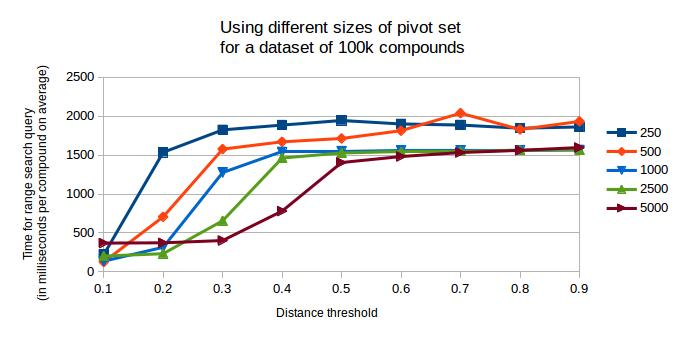
\includegraphics[width=1 \columnwidth]{img/image4.jpg}
\caption{M-tree: Average Range Query time versus Distance Threshold for various sizes of pivot set - 100k PubChem-n database}
\label{fig:5.5}
\end{figure}


We observe that indexing time is increasing almost linearly with increase in the number of pivots chosen at each step of the M-tree algorithm. Even though indexing is an offline process we do not want the indexing time to run into days. If indexing time is very high, updates to the chemical compound database would be very expensive since we need a re-indexing into the chemical database. Hence we need to have a threshold for indexing time.

\begin{figure}[ht!]	
\centering
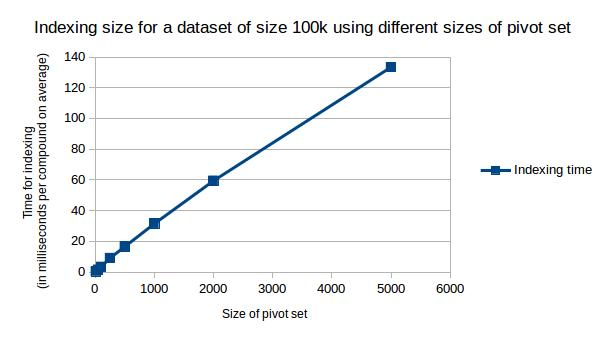
\includegraphics[width=1 \columnwidth]{img/image7.jpg}
\caption{M-tree: Indexing time versus different sizes of pivot set size}
\label{fig:5.6}
\end{figure}



\subsection{Threshold Distance}
As described in earlier sections, the range query distance threshold (t) is thse cutoff used for determining similarity. We observe that range search query time increases monotonically with threshold distance and begins to converge for higher values of threshold distance.  But this seems to hold true only if we use pivots above a particular threshold. 

There are two extremes here. If we use a very high number of pivots most of the time is spent doing computation involving triangle inequality bounds and hence it is not favourable. Similarly if we choose a very low number of pivots, it is not possible to exploit the bounds effectively to decisively prune or include the sub-trees from our answer result set. For low number of pivots used we notice that for high and low values of threshold the query time is lower than that for the middle range, where bounds doesn't help well enough.


As seen in \autoref{fig:5.7}, we observe that for low value of threshold at 0.1, the number of pivots to be chosen seems to have a minima between 500 and 1000 for a dataset size of 100k after which it increases . This is because there is a trade-off between the time saved by pruning the sub-trees versus the time utilized in checking if the nodes can be actually pruned.  For a high threshold value of 0.9 it can be seen that we require more number of pivots . 

\begin{figure}[ht!]	
\centering
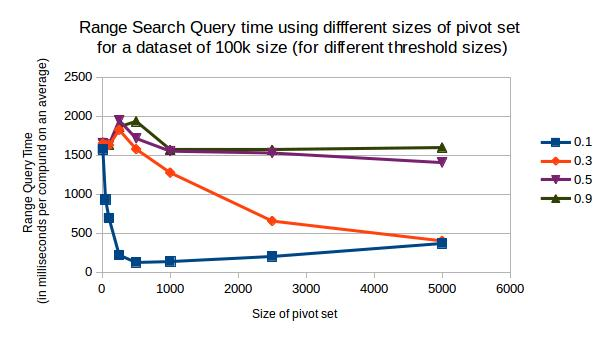
\includegraphics[width=1 \columnwidth]{img/image5.jpg}
\caption{M-tree: Average Range Query time versus various sizes of pivot set for different threshold distances}
\label{fig:5.7}
\end{figure}



\subsection{Dataset Size}
We varied the dataset size for the non-binary version of the PubChem-n to 1000, 10,000 and 100,000 and compared the indexing time as well as range search query time for various thresholds. 


\begin{figure}[ht!]	
\centering
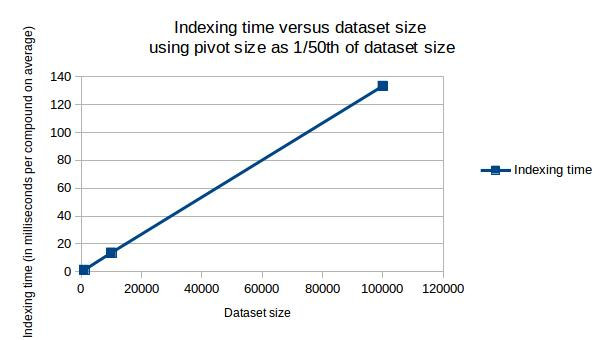
\includegraphics[width=1 \columnwidth]{img/image6.jpg}
\caption{M-tree: Indexing time versus dataset size}
\label{fig:5.8}
\end{figure}

\begin{figure}[ht!]	
\centering
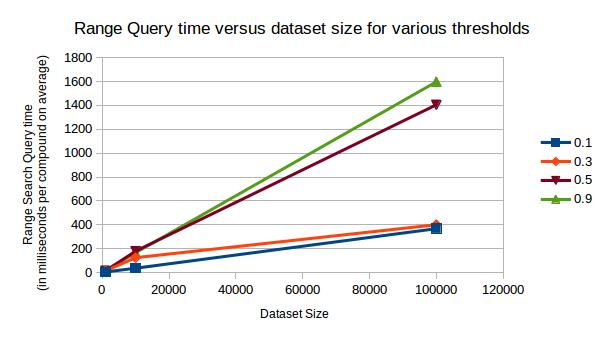
\includegraphics[width=1 \columnwidth]{img/image9.jpg}
\caption{M-tree: Range Query time versus dataset size}
\label{fig:5.9}
\end{figure}


As seen in \autoref{fig:5.9}, we can observe that for a particular value of the distance threshold , the range search query time also increases linearly with dataset size . The slope is higher for higher values of threshold distance.

As seen in \autoref{fig:5.8} we can observe that the average indexing time per compound on average increases linearly with increase in dataset size . This is as a result of our pivoting method with sampling which reduces the computation. If our pivoting step had been an exhaustive search on the database the curve would have not been linear, 





\section{Inverted Indexing Analysis}

For the below experiments the test-bed used was a server with 512GB RAM, 24TB disk space, and 2 quad core Xeon processor. We tested the inverted index structure against both binary as well as non-binary versions of the PubChem-n dataset. For evaluation and verification processes, a complete linear database scan was done as with the M-tree case to compare the result sets. One advantage of Inverted indexing procedure over the M-tree index structure is the much lesser time required for the indexing step. 

Indexing time per compound is observed to be almost constant between 1ms to 2ms per compound on average. As observed in \autoref{fig:5I1} the graph is almost straight parallel to the x-axis for both the binary as well as the non-binary dataset. This is in opposition to the M-tree index structure where the indexing time was increasing with increase in the dataset size. 


\begin{figure}[ht]	
\centering
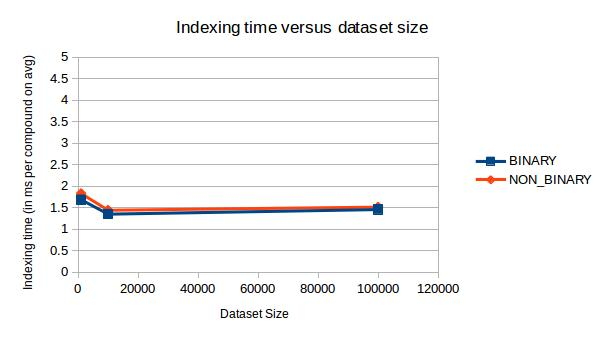
\includegraphics[width=1 \columnwidth]{img/imageI1.jpg}
\caption{Inverted Index: Indexing time versus dataset size for Inverted Indexing}
\label{fig:5I1}
\end{figure}


\autoref{fig:5I2} and \autoref{fig:5I3} show how the range query time graph increases with threshold distances .We can see that in both the figures the time increases monotonically. The double derivative of the curve can be observed to be positive. 

We also observe that the range query time for the binary version of the PubChem-n dataset is lesser compared to the non-binary version of the same dataset. This can be explained by more pruning of features in the binary dataset.

Typically in fingerprint datasets searching is done for a reasonable threshold distance of 0.1 to 0.3 and the search query times uptil 0.3 distance is within a second per compound on average. The figures show that the indexing technique scales well on bigger datasets for low threshold values, better than it scales on higher threshold values.


\begin{figure}[ht]	
\centering
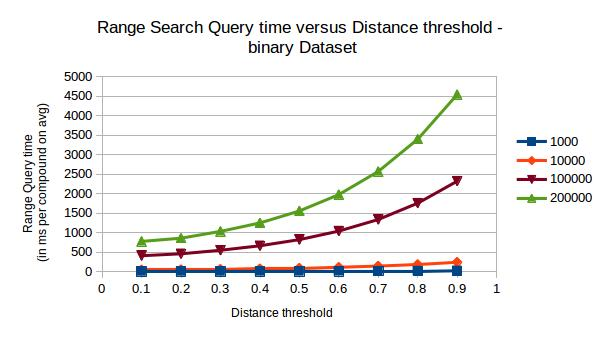
\includegraphics[width=1 \columnwidth]{img/imageI2.jpg}
\caption{Inverted Index: Range Query time versus Distance threshold for different dataset sizes- PubChem-b dataset}
\label{fig:5I2}
\end{figure}

\begin{figure}[ht!]	
\centering
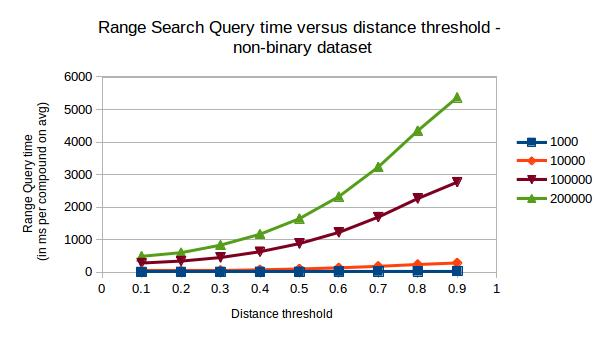
\includegraphics[width=1 \columnwidth]{img/imageI3.jpg}
\caption{Inverted Index: Range Query time versus Distance threshold for different dataset sizes- PubChem-n dataset}
\label{fig:5I3}
\end{figure}


We have also experimented the mentioned improvisations in the Inverted Indexing technique of splitting the heavy hitting features. We observed an increase of about 50-100 ms per compound for the splitting technique.



\section{Comparison of our techniques}

We have compared the three techniques, namely the M-tree indexing technique , the Inverted Indexing technique and the bit bounding technique described in \citet*{swamidass2007bounds}. We have used the PubChem-n, PubChem-b and DUD datasets for our evaluations. A test set of 500 compounds were chosen randomly from the datasets for evaluation purposes. For the experiments, the testbed was a server with 512GB RAM, 24TB disk space, and 2 quad core Xeon processor. 

As observed in \autoref{tab: table1}, comparison of the techniques on the PubChem-b dataset showed for a very low threshold value the M-tree index showed the most promising results, achieving upto two times the speed of the bit bound technique. The inverted index is also able to achieve 2-3 times speed-up compared to the bit bound technique. \\



\begin{table}[ht]
\centering
\caption{Comparsion of techniques applied on the PubChem-n fingerprint dataset}
\label{tab: table1}
\begin{tabular}{|c|c|c|c|}
\hline 
Distance threshold & Mtree	& Bit bound	& 	Inverted Indexing \\
\hline
0.1	& 	386.286549	& 820.3638749	&	485.470212\\
0.2	& 	550.1953386	& 1661.947007	&	596.3910451\\
0.3	& 	2473.023198	& 2524.738663	&	826.6685434\\
0.4	& 	4936.808636	& 3363.817437	&	1162.332165\\
0.5	& 	5063.290607	& 4090.751155	&	1643.795028\\
0.6	& 	5122.609976	& 4654.190322	&	2321.426377\\
0.7	& 	5145.041938	& 5018.220471	&	3230.933406\\
0.8	& 	5152.297697	& 5175.073409	&	4346.756728\\
0.9	& 	5178.022697	& 5229.718132	&	5371.661469\\
\hline 
\end{tabular} 
\end{table}

We have shown the effectiveness of out technique on non-binary datasets, a feature unexplored in most papers in the field of research. We can observe from the \autoref{tab: table1} that for high values of distance threshold all three techniques start converging to similar runtime for the range search query. \\

\begin{table}[ht!]
\centering
\caption{Comparsion of techniques applied on the PubChem-b fingerprint dataset}
\label{tab: table2}
\begin{tabular}{|c|c|c|c|}
\hline 
Distance threshold & Mtree	& Bit bound	& 	Inverted Indexing \\
\hline
0.1 & 384.8059272 	&	708.6588827 	&	776.7649653\\
0.2 & 480.429907	  	&  	1444.478385	&	859.3060838\\
0.3 & 1941.113211 	&	2217.534745 	&	1033.699747\\
0.4	& 4896.263139 	&	2995.191962 	&	1251.065067\\
0.5	& 5037.030643 	&	3736.857438 	&	1556.630309\\
0.6	& 5086.700389 	&	4354.433042 	&	1976.196625\\
0.7	& 5118.526736 	&	4859.848535 	&	2568.638003\\
0.8	& 5138.21594	 	& 	5082.24385 	&	3396.452903\\
0.9	& 5168.943088	&	5138.640137 	&	4540.309089\\
\hline 
\end{tabular} 
\end{table}




\begin{table}[ht!]
\centering
\caption{Comparsion of techniques applied on the binary DUD dataset}
\label{tab: table3}
\begin{tabular}{|c|c|c|c|}
\hline 
Distance threshold & Mtree	& Bit bound	& 	Inverted Indexing \\
\hline
0.1 	& 107.1823181	& 146.6163294	& 	29.37458224\\
0.2 & 297.8381414	& 217.9150917	& 	35.10997253	\\
0.3 & 303.2994695	& 272.7101361	& 	39.32821769	\\
0.4 & 295.2179914	& 292.4566623	& 	43.20251988	\\
0.5 & 299.248134 	& 304.6924106	& 	56.92043218	\\
0.6 & 297.995192 	& 294.1471833	& 	69.95566644	\\
0.7 & 289.2738744	& 295.0616706	& 	91.30182238	\\
0.8	& 301.1660971	& 287.0035369	& 	127.5203695	\\
0.9 & 294.3855533	& 289.8519661	& 	191.9871398	\\
\hline 
\end{tabular} 
\end{table}


\autoref{tab: table2} shows the comparison of techniques applied on the PubChem-b dataset while \autoref{tab: table3} shows the comparison of the techniques on the binary DUD dataset. The performance of M-tree index can be seen to be comparable to the bit bound while the performance of the inverted index can be observed to be superior than both the other techniques. For the PubChem-b dataset we observe  that there is always a 2-2.5 times speedup for the inverted index as compared to the bit bound technique. The M-tree index beats the other two techniques for low threshold values but there is a sharp increase in range search query time around 0.3 where the runtime shoots up .


\begin{figure}[ht!]	
\centering
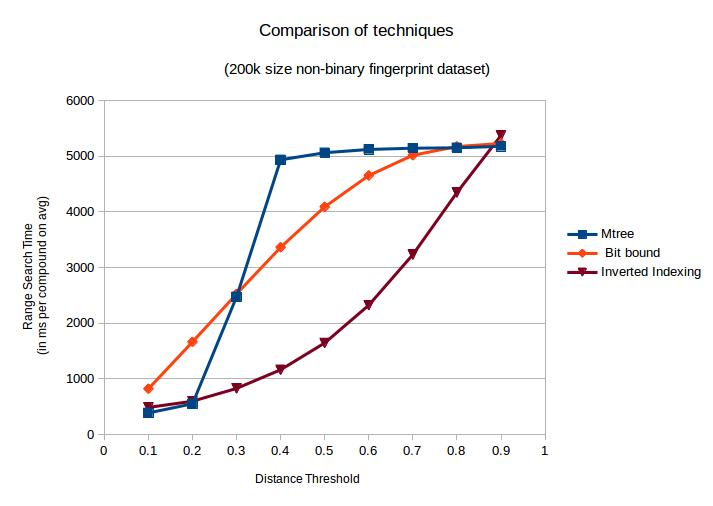
\includegraphics[width=0.75 \columnwidth]{img/imageC1.jpg}
\caption{Comparsion of techniques applied on the PubChem-n fingerprint dataset}
\label{fig:5C1}
\end{figure}


Comparison on the DUD dataset showed that the inverted indexing technique was able to achieve 5-6 times speedup on the M-tree index and the bit bound algorithm. As observed in \autoref{fig:5C1}, \autoref{fig:5C2} and \autoref{fig:5C3} our inverted indexing technique works better than the other two on an average. The M-tree technique works well for lower threshold values, sometimes better than the inverted index technique but fails to scale for higher threshold values. 



\begin{figure}[ht]	
\centering
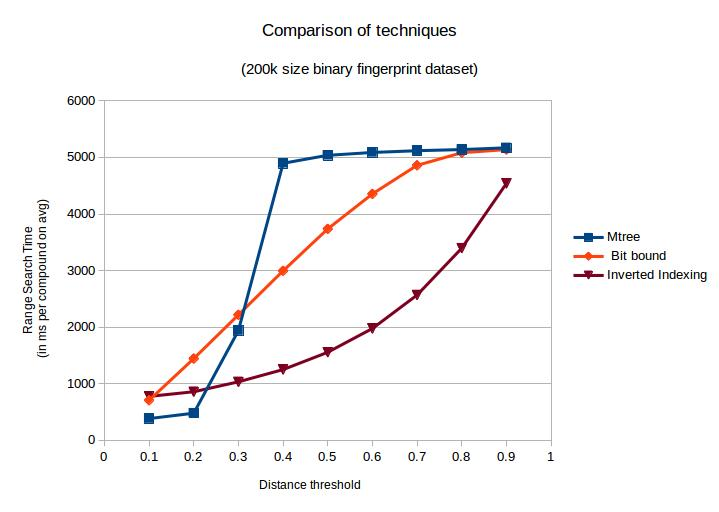
\includegraphics[width=0.75 \columnwidth]{img/imageC2.jpg}
\caption{Comparsion of techniques applied on the PubChem-b fingerprint dataset}
\label{fig:5C2}
\end{figure}

\begin{figure}[ht!]	
\centering
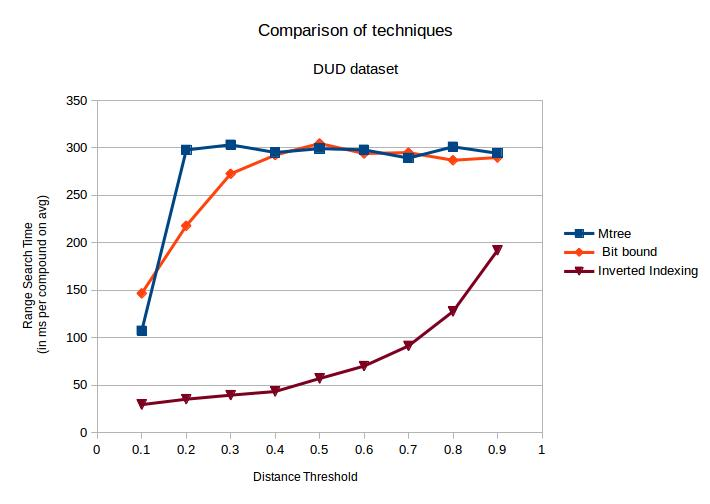
\includegraphics[width=0.75 \columnwidth]{img/imageC3.jpg}
\caption{Comparsion of techniques applied on the binary DUD dataset}
\label{fig:5C3}
\end{figure}

Comparing the M-tree index structure with inverted index technique, we observe the following: The indexing time  per compound on average is constant for the inverted index structure while it varies linearly with size of the dataset for the M-tree. The run-times for range search queries tends to converge for both the methods as we go towards higher threshold values. The M-tree index shows a sudden increase in runtime for range query at around 0.3 while the curve for the inverted index is smoother. Also, if we were to include a new point into the chemical database the inverted index structure would be simpler since we would just need to update the corresponding feature lists while we would have to undergo a re-indexing for the M-tree index since it would be difficult to add the point randomly into the tree structure.

